Hello world! the following text is in Spanish: \textspanish{Me gusta el diseño gráfico}.
\begin{enumerate}
 \item 
 This is an example using a lot of mathematics an equations. 
 First, we show that we can create a simple equation like this:
 \begin{equation}
 \label{eq:elipse}
 \frac{x^{2}}{a^{2}} + \frac{y^{2}}{b^{2}} = 1
 \end{equation}
 And we can refer to it later in the text like this: the equation \eqref{eq:elipse} is an elipse.
 If we do not want to have it numbered we can say:
 \begin{equation}
 \nonumber
 \binom{n}{k} = \frac{n!}{k!(n-k)!} 
 \end{equation}
 And you can also embed equations into text for example: $\forall x \in \mathbb{R}$. 
 You can make links to an externam website like this: 
 To learn how to use the sumation and integrals you can check the \href{https://en.wikibooks.org/wiki/LaTeX/Mathematics#Sums_and_integrals}{wikibooks} in or search for it in \url{www.google.com}.
 The last form makes the link use other font.
 
 \item This is an example of an function with cases, like a \emph{pdf}.
 \begin{equation}
  \label{eq:pdf}
  f(y) =
  \begin{cases}
    \frac{1}{25} y & \quad \text{if } 0 \leq y < 5 \\
    \frac{2}{25} - \frac{1}{25} y & \quad \text{if } 5 \leq y < 10 \\
    0 & \quad \text{if } y < 0 \text{ or } y > 10
  \end{cases}
 \end{equation}
 This is an example of automatic sizing parenthesis:
 \begin{equation}
  \nonumber
  P\left(A=2\middle|\frac{A^2}{B}>4\right)
 \end{equation}
 And finally, an example of making math in several steps uisng the \verb|align| enviroment.
 With $*$ in the enviroment you omit the numbers
\begin{align*}
P\left(X \leq 3 \right) &= \int_{0}^{3} \frac{1}{25} y \,\mathrm{d}y \\
     &= \left. \frac{1}{25} \cdot \frac{1}{2} \, y^{2} \right|_0^3 \\
     &= \frac{1}{25} \left( \frac{1}{2} \, 9 - \frac{1}{2} \, 0 \right) =
     \frac{1}{25} \cdot \frac{9}{2} = \frac{9}{50} \approx 0.18 
\end{align*}

 \item This section shows how to place figures.
 The most common way is to place a figure centered with his caption.
 
\begin{figure}[htb]
  \centering
  \label{fig:one}
  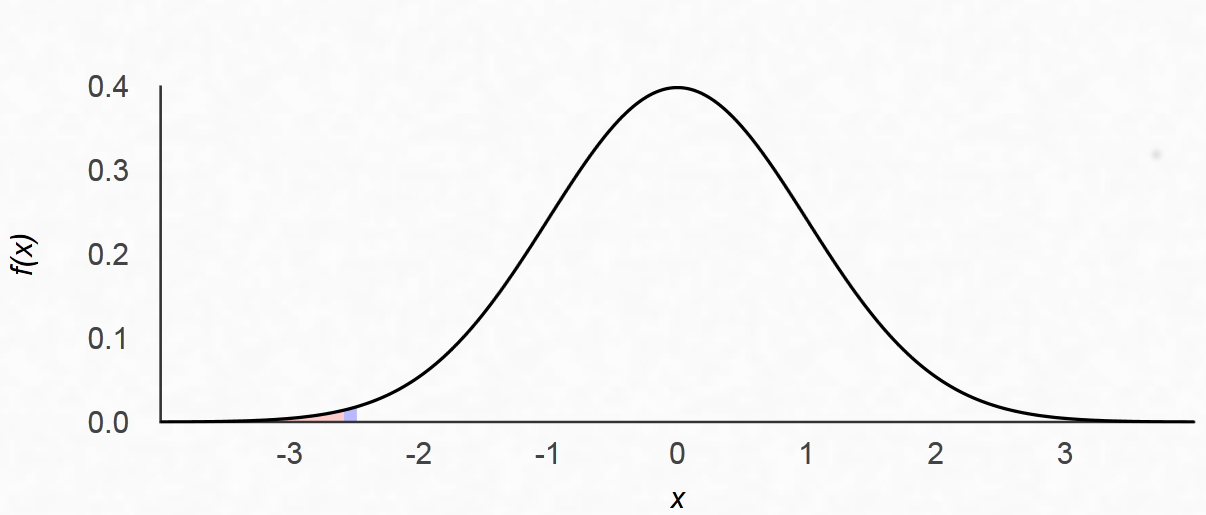
\includegraphics[width=0.4\textwidth]{img/normal}
  \caption{Plot of nomral distribution from \href{https://www.statmethods.net/advgraphs/probability.html}{R scrip}.}
\end{figure}

But its also possible to have a figure that is composed of several subfigures.
Each subfigure with his caption and an extra caption for the whole figure group.
And then you can reference them like this: See Figure~\ref{fig:two} or refer to subfigure like this: See Sub Figure~\ref{fig:2b}.

\begin{figure}[htp]
  \centering
  \begin{subfigure}[b]{0.3\textwidth}
    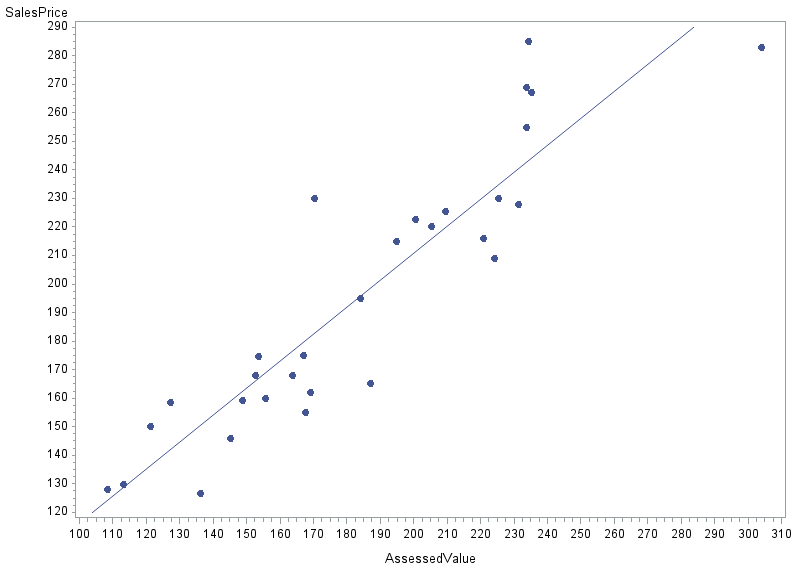
\includegraphics[width=\textwidth]{img/scatter}
    \caption{Scatter plot Assessed value v.s. sales price.}
  \label{fig:2a}
  \end{subfigure}
    ~
  \begin{subfigure}[b]{0.3\textwidth}
    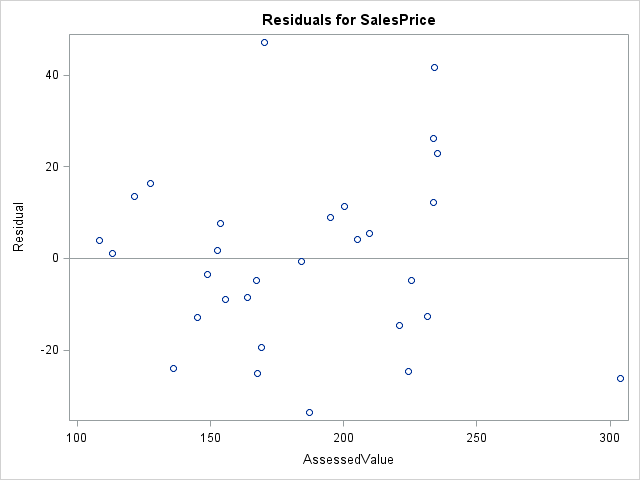
\includegraphics[width=\textwidth]{img/residuals}
    \caption{Residuals vs assesed value.}
    \label{fig:2b}
  \end{subfigure}
  ~
  \begin{subfigure}[b]{0.3\textwidth}
    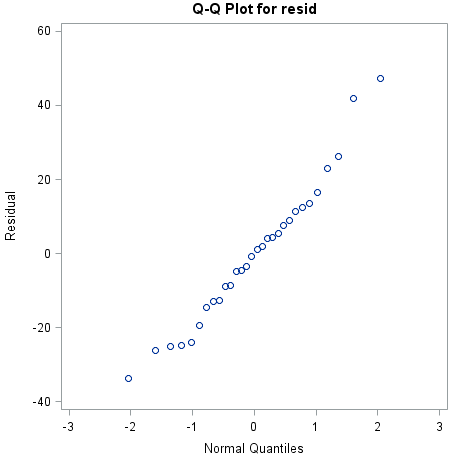
\includegraphics[width=\textwidth]{img/qqplot}
    \caption{Normal quantile plot of the residuals.}
    \label{fig:2c}
  \end{subfigure}
    
  \caption{Plots of an imaginary exercise, lets call it $X$.}
  \label{fig:two}
\end{figure}

\item This is an example of how to cite a book.: this exercise was taken from~\cite{Devore2012}. 
We also show an example of how to put a book in the references without actually citing it. 
And finally, this is an example of a very nice table: Table \ref{tab:exey}

\begin{table}[htb]
  \begin{center}
    \begin{tabular}{l | r r r r r}
      \toprule
      Source & \textbf{DF} & \textbf{SS} & \textbf{MS} & \textbf{F} & \textbf{P-value} \\
      \midrule
      \textbf{Model} & 2 & 0.00318564 & 0.00159282 & 7.72 & 0.0014 \\
      \textbf{Error} & 42 & 0.00866760 & 0.00020637 &  & \\
      \midrule
      \textbf{Total} & 44 & 0.01185324 &   &  & \\
      \bottomrule
    \end{tabular}
  \end{center}
\caption{Anova table for an imaginary exercise}
\label{tab:exey}
\end{table}

\item In this number lets look at how to write an algorith using pseudo code.
See the algorithm~\ref{alg:euclid}. The while ends in line~\ref{euclidendwhile}.
The information comes from this part of the \href{https://en.wikibooks.org/wiki/LaTeX/Algorithms#Typesetting_using_the_algorithmicx_package}{wikibook} and from this \href{https://tex.stackexchange.com/questions/229355/algorithm-algorithmic-algorithmicx-algorithm2e-algpseudocode-confused}{post}.

The algorithm enviroment uses all the width of the page.
There is a \href{https://tex.stackexchange.com/questions/350434/adjust-width-of-algorithm-float}{hack} to make it fit into a certain width, however use it with caution.

{\centering
\begin{minipage}{\linewidth}
  \begin{algorithm}[H]
    \caption{Euclid's algorithm}
    \label{alg:euclid}
    \begin{algorithmic}[1] % The number tells where the line numbering should start 0 for no number
      \Procedure{Euclid}{$a,b$} \Comment{The g.c.d. of $a$ and $b$}
        \State $r\gets a \bmod b$
        \While{$r\not=0$} \Comment{We have the answer if $r = 0$}
          \State $a \gets b$
          \State $b \gets r$
          \State $r \gets a \bmod b$
        \EndWhile\label{euclidendwhile}
        \State \textbf{return} $b$\Comment{$gcd = b$}
      \EndProcedure
    \end{algorithmic}
  \end{algorithm}
\end{minipage}
\par
}

\item Here we show how include surce code using the package minted. We are going to show an example in the C language.
\begin{minted}{c}
int main() {
  printf("hello, world");
  return 0;
}
\end{minted}

This is another example; this time on the \emph{R language}

\begin{minted}{R}

 A <- matrix(c(0.15, 0.01, 0,
               0.14, 0.36, 0.07,
               0.15, 0.13, 0.3), ncol = 3, byrow = TRUE)
 I = diag(nrow = nrow(A))

 I%*%A
\end{minted}

This is yet another example of inlined Python code: \mintinline{python}{print(x**2)} lets see how it looks.
Finally, lets try to input another file: See Listing \ref{lst:example}.
I took a lot of help from \href{https://tex.stackexchange.com/questions/252263/alignment-of-minted-line-numbers}{here} and \href{https://www.overleaf.com/learn/latex/Code_Highlighting_with_minted}{Overleaf help}.
We are using the same hack that we used with the algorithm to make the listing fit into the margins.

{\centering
\begin{minipage}{\linewidth}
  \begin{listing}[H]
  \inputminted[
  xleftmargin=1.5cm,  %without this option line number goes wrong
  %frame=lines,
  framesep=0.5cm,
  baselinestretch=1.2,
  %fontsize=\footnotesize,
  linenos,
  firstline=54, %If you omit this two fields, the whole file is pulled
  lastline=68
  ]{cpp}{src/GccTest.cpp}
  \caption{My buggy implementation of insertion sort. (Do not use)}
  \label{lst:example}
  \end{listing}
\end{minipage}
\par
}

\end{enumerate}
